\documentclass[french, 11pt]{article} 

%=================================================
% Packages and New Commands
%=================================================

%===== Packages ==================================
%=================================================

\usepackage[utf8]{inputenc}

\usepackage[]{afterpage}
\usepackage[]{amsfonts}
\usepackage[]{amsmath, amssymb}
\usepackage[toc, page]{appendix}
\usepackage[french, english]{babel}
\usepackage[citestyle=verbose-trad2, bibstyle=numeric, sorting=nty]{biblatex}
\usepackage[]{blindtext}
\usepackage[]{booktabs}				% Better tables.
\usepackage[]{caption}
\usepackage[]{chngcntr}
\usepackage[]{csquotes}
\usepackage[]{enumitem}
\usepackage[]{etoolbox}
\usepackage[]{fancyhdr}				% Page headers package.
\usepackage[]{float}
\usepackage[T1]{fontenc}
\usepackage[]{fontspec}
\usepackage[]{gensymb}
\usepackage[a4paper, total={162mm,245mm}, top=28mm]{geometry}
\usepackage[]{graphicx}
\usepackage[]{hyperref}
\usepackage[]{lastpage}
\usepackage[]{layout}
\usepackage[]{listings}				% Code insert package.
\usepackage[]{lmodern}
\usepackage[]{lscape}
\usepackage[]{makecell}
\usepackage[]{mathtools}
\usepackage[]{mathrsfs}
\usepackage[]{mdframed}
\usepackage[]{multicol}
\usepackage[]{multirow}
\usepackage[nottoc]{tocbibind}
\usepackage[]{parskip}
\usepackage[]{pdfpages}
\usepackage[]{pgfplots}
\usepackage[]{soul}
\usepackage[]{subcaption}
\usepackage[]{titlesec}
\usepackage[normalem]{ulem}
\usepackage[]{url}
\usepackage[]{wrapfig}
\usepackage[]{xcolor}

%===== New Commands ==============================
%=================================================

% New command to create a blank page without it being counted on the total page count.
\newcommand{\blankpage}
{
	\null
	\thispagestyle{empty}
	\addtocounter{page}{-1}
	\newpage
}

\newcommand{\question}[1]
{
	\vspace{0.3cm}
	\begin{mdframed}[style=Question]
		#1
	\end{mdframed}
}

\newcommand{\CMDblock}[1]
{
	{\colorbox{black!15}{\texttt{#1}}}
}

\newcommand{\HESSo}{HES$\cdot$So\xspace}
\newcommand{\HESGe}{HES$\cdot$Ge\xspace}

\newcommand{\DocVersion}{1.0.0}

\newcommand{\DocTitle}{Projet Asseto Corsa}
\newcommand{\DocSubject}{Microcontrôleurs et Périphériques}

\newcommand{\SubjectProfessor}{M. Abegg Christian\xspace}

% Make \paragraph as a subsubsubsection
\makeatletter
\renewcommand{\paragraph}{\@startsection{paragraph}{4}{0ex}%
   {-3.25ex plus -1ex minus -0.2ex}%
   {1.5ex plus 0.2ex}%
   {\normalfont\normalsize\bibfont\bf}}
\makeatother

% Make \paragraph appear in TOC
\stepcounter{secnumdepth}
\stepcounter{tocdepth}

%=================================================
% Themes, Colors and Styles
%=================================================

\lstset{
    backgroundcolor=\color{ltGrey2},
    aboveskip=3mm,
    belowskip=3mm,
    framexleftmargin = 1em,
    showstringspaces=false,
    columns=flexible,
    basicstyle={\small\ttfamily},
    numbers=none,
    numberstyle=\tiny\color{gray},
    keywordstyle=\color{dkRed},
    commentstyle=\color{ltGrey},
    stringstyle=\color{orange-yellow},
    breaklines=true,
    breakatwhitespace=false,
    tabsize=3
}

\usepackage{color}
\definecolor{dkRed}{RGB}{204,0,0}
\definecolor{ltGrey}{RGB}{150,150,150}
\definecolor{ltGrey2}{RGB}{240,240,240}
\definecolor{orange-yellow}{RGB}{250,200,0}


\mdfdefinestyle{Question}{backgroundcolor = black!5, linecolor=black!10, linewidth=2pt}

\renewcommand*{\lstlistingname}{Extrait de code}
\renewcommand*{\lstlistlistingname}{Table des extraits de code}

%=================================================
% Packages Configuration
%=================================================

\hypersetup
{
	bookmarksopen=true,
	pdftitle="\DocTitle\ - \DocSubject",
	pdfauthor="Joachim Bach ; David Da Silva Marques",
	pdfsubject="Bachelor I.S.C",
	pdftoolbar=true,				% Toolbar hidden.
	pdfpagemode=UseOutlines,
	pdfstartview={Fit},				% Fits the width of the page to the window.
	pdfmenubar=true,
	pdfhighlight=/O,
	colorlinks=true,
	pdfpagelayout=OneColumn,
	pdffitwindow=false,
	linktoc=section,
	linkcolor=blue,
	citecolor=blue,
	urlcolor=blue,
}

\bibliography{Others/Bibliography.bib}

\AtEveryCitekey
{
	\clearfield{urldate}
}

%=================================================
% Document Details - Preamble
%=================================================

\title{\DocSubject}
\author{Joachim BACH ; David DA SILVA MARQUES}
\date{\today}

\makeatletter
\let\TheTitle\@title
\let\TheAuthor\@author
\let\TheDate\@date
\makeatother

\pagestyle{fancy}
\fancyhf{}
\lhead{ \textsc{HEPIA Genève} \\ \DocSubject}
\rhead{ \textsc{version} \DocVersion \\ \TheDate}
\cfoot{\thepage \hspace{0.1 mm} / \pageref*{LastPage}}

%=================================================
%=================================================
%=================================================
% Start Document
%=================================================
%=================================================
%=================================================



\begin{document}
	
	\selectlanguage{french}
	\normalsize
	
	\begin{titlepage}
		
		\centering
		\vspace*{2.0 cm}
		
		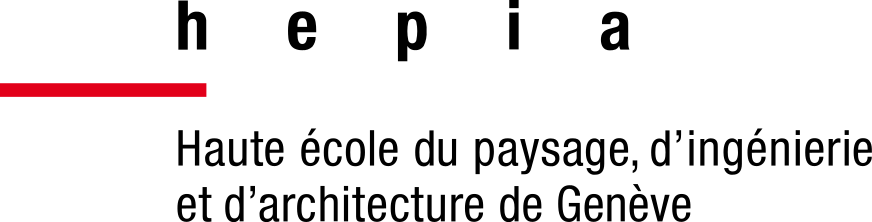
\includegraphics[scale = 1.50]{Images/HEPIA_Logo.png}\\[1.0 cm]
		
		\vspace{1.0 cm}
		
		\rule{\linewidth}{0.3 mm} \\[0.2 cm]
		{\Huge \textbf{\DocTitle}}\\
		\vspace{4 mm}
		{\huge \TheTitle}\\
		\rule{\linewidth}{0.3 mm} \\[1.2 cm]
		
		\textsc{\Large Bachelor I.S.C}\\[0.5 cm]
		
		\vspace{1.5 cm}
		
		\begin{minipage}{0.40\textwidth}
			
			\begin{flushleft}
				\Large\emph{Auteur(s) :}\\[0.2 cm]
				\Large\emph{}\\[0.2 cm]
				\Large\emph{}\\[0.2 cm]
				\Large\emph{}\\[0.2 cm]
				\Large\emph{Institution :}\\[0.2 cm]
				\Large\emph{Date :}\\[0.2 cm]
				\Large\emph{Version :}\\[0.2 cm]
				\Large\emph{Professeur-re :}\\[0.2 cm]
			\end{flushleft}
		
		\end{minipage}~
		\begin{minipage}{0.53\textwidth}
			
			\begin{flushright}
				\Large{Joachim Bach (22650667)}\\[0.2 cm]
				\Large{David Da Silva Marques (226449792)}\\[0.2 cm]
				\Large\emph{}\\[0.2 cm]
				\Large{HEPIA Genève}\\[0.2 cm]
				\Large{\TheDate}\\[0.2 cm]
				\Large{\DocVersion}\\[0.2 cm]
				\Large{\SubjectProfessor}\\[0.2 cm]
			\end{flushright}
		
		\end{minipage}
	
	\end{titlepage}
	
	\blankpage

	{\hypersetup{hidelinks} \tableofcontents}
	
	\pagebreak
	
	{\hypersetup{hidelinks} \listoffigures}
	
	\addcontentsline{toc}{section}{Table des extraits de code}
	{\hypersetup{hidelinks} \lstlistoflistings}
	
	\pagebreak

    \section{Introduction}

    Dans le cadre du cours Microcontrôleur et Périphériques (MIPS), nous avons dû réaliser un projet. Celui-ci a pour but, et exigences, de réunir l'ensemble des interfaces et fonctionnalités étudiées durant ce semestre.

    La contrainte principale est que nous devions utiliser deux cartes MyLab2. Nous avions aussi pour obligation d'utiliser les interfaces suivantes :

    \begin{enumerate}
        \item CAN
        \item Écran avec texte
        \item Communication UART
        \item Dalle tactile
        \item SysTick / Timer
        \item Boutons
    \end{enumerate}

	Le code doit être le même sur les deux cartes, la différence se faisant au lancement en fonction de la position du dipswitch 0.

    \subsection{Présentation du projet}

    Le projet que nous avons choisi consiste à développer une sorte de manette de jeu pour jouer au simulateur de course automobile "Assetto Corsa". 
	
	Voici une description de l'utilisation des deux MyLab2 : 
	Une des deux cartes sert de volant, grâce à l'accéléromètre, avec des boutons pour l'accélérateur et le frein. Les LEDS du dipswitchs sont utilisées comme indicateur de compte-tours. L'autre carte sert de tableau de bord affichant la télémétrie du jeu et ayant un ensemble de boutons pour permettre quelques inputs supplémentaires.

	% //TODO add final physical image of the setup

    \section{Architecture}

		Dans cette section de notre rapport, nous allons présenter les différentes parties composant notre périphérique. Il s'agira de discuter de la partie PC, de la carte servant de volant ainsi que de celle servant de tableau de bord.

		\subsection{Schéma de l'architecture}

			Voici un schéma conceptuel décrivant l'architecture mise en place dans le cours de ce travail pratique :

			\begin{figure}[H]
				\centering
				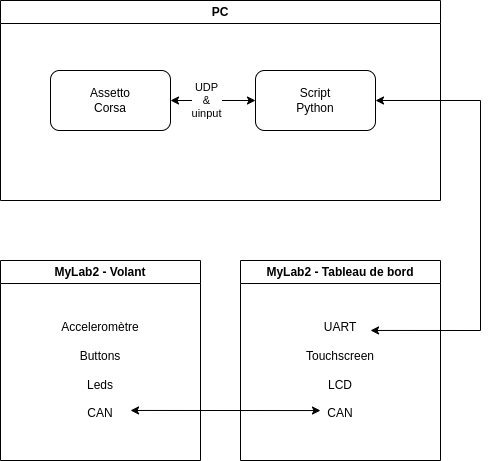
\includegraphics[width=0.55\textwidth]{Images/architecture.drawio.png}
				\caption{Schéma de l'architecture}
			\end{figure}
			
        \subsection{Implémentation côté PC}

        Du côté du PC se trouve Assetto Corsa, un jeu de voiture ainsi qu'un script python tournant en arrière-plan. Ce script python se charge de récupérer la télémétrie d'Assetto Corsa à travers un socket UDP mis à disposition par le jeu (il s'agit d'une méthode d'accès à la télémétrie courante dans le monde des simulateurs). Le python récupère alors les informations qui l'intéressent et les envoie sur l'UART vers le "Tableau de bord", autrement dit l'une des deux cartes. 
		
		Depuis cette même connexion UART, le script récupère les inputs (inclinaison du volant, pression des boutons, etc.) sous forme de tableau d'octets envoyé par la carte tableau de bord. Ces informations sont ensuite transmises à une classe "Gamepad" qui simule un périphérique qui est ensuite utilisée par le jeu comme un n'importe quel autre périphérique/manette/etc et qui est ainsi utilisable en jeu.

		Le script gère les coupures de connexion avec le jeu et/ou la carte, tout comme les cartes gèrent les pertes de connexion entre elles et avec le PC, affichant la situation actuelle à l'utilisateur de la manière suivante:

		```
		AC TELEMETRY & VIRTUAL GAMEPAD:
		-------------------------------------

		Assetto Corsa link : NOT CONNECTED                         
		Dashboard link     : NOT CONNECTED   
		```

		Les états possibles pour "Assetto Corsa link" sont:

		\begin{enumerate}
			\item "NOT CONNECTED", la connection n'a pas encore été établie
			\item "TRYING HANDSHAKE", le script tente de faire un handshake avec Assettot Corsa dans le but de recevoir les données de télémetrie
			\item "TIMEOUT", le script n'as pas reçu de réponse de la part d'Assetto Corsa depuis un moment, indiquant que le jeu s'est arrêté ou qu'il y a un problème
			\item "CONNECTED". le script reçoit les données correctement
		\end{enumerate}

		Les états possibles pour "Dashboard link" sont: 

		\begin{enumerate}
			\item "NOT CONNECTED", le câble UART n'est pas branché
			\item "RESETING", le script se reset pour corriger un problème de mismatch avec le dashboard 
			\item "TIMEOUT", le script n'a pas reçu de donnée du dashboard depuis un moment
			\item "CONNECTED". le script reçoit les inputs du dashboard correctement
		\end{enumerate}

		% //TODO mettre une image du jeu avec le script qui toure à côté

		\subsubsection{Détails du protocole entre le PC et le tableau de bord}
		\label{telemetrie}

			Le code python s'exécutant sur le PC être chargé d'à la fois envoyer les données de télémétrie mais aussi de recevoir les inputs provenant du tableau de bord.

			Pour l'envoi de la télémétrie, il envoie en UART un ensemble de données de télémétrie récupérées via le port UDP du jeu. Voici l'ensemble des données composant une trame :

			\begin{lstlisting}[language=python, caption=Données télémétriques envoyées par le python]
uart.serial_send(struct.pack("?", False)) #reset screen bool
uart.serial_send(struct.pack("f", live_data['speed_Kmh']))
uart.serial_send(struct.pack("I", live_data['lapTime']))
uart.serial_send(struct.pack("f", live_data['wheelAngularSpeed_0']))
uart.serial_send(struct.pack("f", live_data['gas']))
uart.serial_send(struct.pack("f", live_data['brake']))
uart.serial_send(struct.pack("I", int(live_data["engineRPM"])))
uart.serial_send(struct.pack("?", live_data['isAbsEnabled']))
uart.serial_send(struct.pack("?", live_data['isTcEnabled']))
uart.serial_send(struct.pack("I", message_counter))
			\end{lstlisting}

			Du côté du tableau de bord, la réception de l'UART se charge de remplir une structure contenant toutes les informations nécessaires à un traitement de données (une sorte de trame complète).

			Voici le contenu de cette "trame" : 

			\begin{lstlisting}[language=c, caption=Contenu d'une "trame" de données télémétriques côté tableau de bord]
typedef struct __attribute__ ((__packed__)) _uart_telemetry
{
	bool stop_display;
	float speed_kmh;
	uint32_t lap_time;
	float wheel_angular_speed_0;
	float gas;
	float brake;
	uint32_t engine_RPM;
	bool is_abs_enabled;
	bool is_tc_enabled;
	uint32_t message_counter;
}uart_telemetry;
			\end{lstlisting}

		
			Une donnée supplémentaire envoyée par le python est le "message\_counter". Cela permet au tableau de bord de détecter une erreur, dans le cas ou le message counter n'est pas le même que le sien, et ainsi provoquer un reset de la communication. Cela peut arriver si le script python n'est pas correctement synchronisé avec le tableau de bord, entrainant un remplissage erroné de la structure d'une trame.

			Le code python peut aussi demander au tableau de bord de se réinitialiser, dans le cas ou, par exemple, l'utilisateur quitte une course. En effet, si le jeu ne s'exécute plus, les données de télémétrie ne sont plus envoyées et il faut alors "nettoyer" les écrans du tableau de bord et du volant afin qu'ils n'affichent pas de données erronées.


			Il est très important de noter qu'il y a une limite à la vitesse d'envoi du python, qu'il est très important de ne pas dépasser. Cette limite est assurée par la variable globale suivante : 

\begin{lstlisting}[language=python, caption=Variable de ralentissement de l'envoi des données par le python]
MESSAGE_SENT_WAIT_MICROSECONDS = 100000
\end{lstlisting}

		Si l'envoi devient trop rapide, il est possible que le tableau de bord n'arrive pas à suivre et doive alors se réinitialiser en permanance.

        \subsection{MyLab2 Volant}

		La carte MyLab2 servant de volant est celle tenue entre les mains du joueur. Son rôle est de simuler un volant de course et doit ainsi permettre de guider la voiture, mais aussi de contrôler l'accélérateur, les freins et d'afficher quelques informations sur la voiture.

        Le volant s'occupe alors de récupérer les valeurs de son accéléromètre et de les convertir en un angle. Il envoie en continu le résultat de ce calcul par CAN à a carte servant de tableau de bord. Lors de l'appui sur le bouton A ou B, un message CAN est transmis immédiatement au tableau de bord. 
		
		Le volant reçoit sur le CAN, les RPM du moteur et la vitesse de la voiture. Ceux-ci seront affichés respectivement sur les LEDS des dipswitchs et sur le LCD sous forme de cadrant avec une aiguille. 

		\subsubsection{Modifications du protocole CAN}
		\label{CAN}

		Le protocole CAN a été légèrement modifié afin d'ajouter une zone de commande ainsi qu'une zone de données dans chaque message. Les 8 premiers bits sont utilisés pour signaler la commande utilisée. Cela permet de faire un traitement en fonction du type de message reçu. Voici l'exemple de la réception CAN du volant : 

\begin{lstlisting}[language=c, caption=Exemple de réception CAN en fonction du champ de commande]
uint32_t received_id;
uint8_t* received_data;

can_get_message(&received_id, &received_data);

if(received_data[0] == CAN_SPEED_DATA_NUMBER)
{
	uint32_t speed = (received_data[1] + (received_data[2] << 8) + (received_data[3] << 16) + (received_data[4] << 24));
	gui_draw_speed(80, 30, speed);

	gui_draw_speedometer(120, 160, 80, speed);
}
else if(received_data[0] == CAN_RPM_DATA_NUMBER)
{
	uint32_t engine_RPM = (received_data[1] + (received_data[2] << 8) + (received_data[3] << 16) + (received_data[4] << 24));

	gui_display_shift_indicator_leds(engine_RPM, CAR_MAX_RPM);
}
\end{lstlisting}


		Voici l'ensemble des commandes différentes possibles actuellement : 

\begin{lstlisting}[language=c, caption=Liste des commandes CAN disponibles]
#define CAN_RESET_CMD_NUMBER 0
#define CAN_SPEED_DATA_NUMBER 1
#define CAN_BTN_A_DATA_NUMBER 2
#define CAN_BTN_B_DATA_NUMBER 3
#define CAN_RPM_DATA_NUMBER 4
#define CAN_WHEEL_ROTATION 5
\end{lstlisting}

		% //TODO mettre une image de près du volant
        
        \subsection{MyLab2 Tableau de bord}

        Le tableau de bord est la pièce centrale du projet : cette carte sert d'intermédiaire entre le volant et le PC. Le tableau de bord reçoit à travers l'UART (Ref section \ref{telemetrie}) la télémétrie venant du jeu, dont il affiche l'accélérateur et le frein, mais aussi le temps du tour (lap time). Il retransmet ensuite la vitesse et les RPM au volant via CAN (Ref section \ref{CAN}). De celui-ci il récupère la rotation et les boutons, qu'il stocke dans un tableau local. Toutes les 20ms, il envoie alors ce tableau par la même connexion UART pour que le PC puisse interpréter les inputs. 

        \subsection{Matériel}    

        Pour ce projet nous avons donc besoin :

        \begin{enumerate}
            \item 1 PC avec Assetto Corsa et 1 script python permettant d'interfacer avec les cartes
            \item 2 MyLab2 + LPC1769
            \item 1 câble USB A → micro-USB
            \item 1 câble CAN
            \item Câbles d'alimentation
        \end{enumerate}


	\section{Problèmes rencontrés}

	Initialement il avait été prévu que les cartes soient utilisé en tant périphériques USB. Cependant, il s'avère que c'est un protocole relativement sensible et précis, rendant compliqué son implémentation dans un délai aussi court. Heureusement un plan de secours avait été prévu, utiliser un script python couplé à de l'UART pour la transmission des données pour pouvoir simuler un périphérique logiciellement. Cependant, cette solution n'est pas miraculeuse et ne fonctionne pas de manière stable.

    \section{Conclusion}



\end{document}